\documentclass{standalone}
\usepackage{tikz}
\usetikzlibrary{patterns, positioning}

\begin{document}
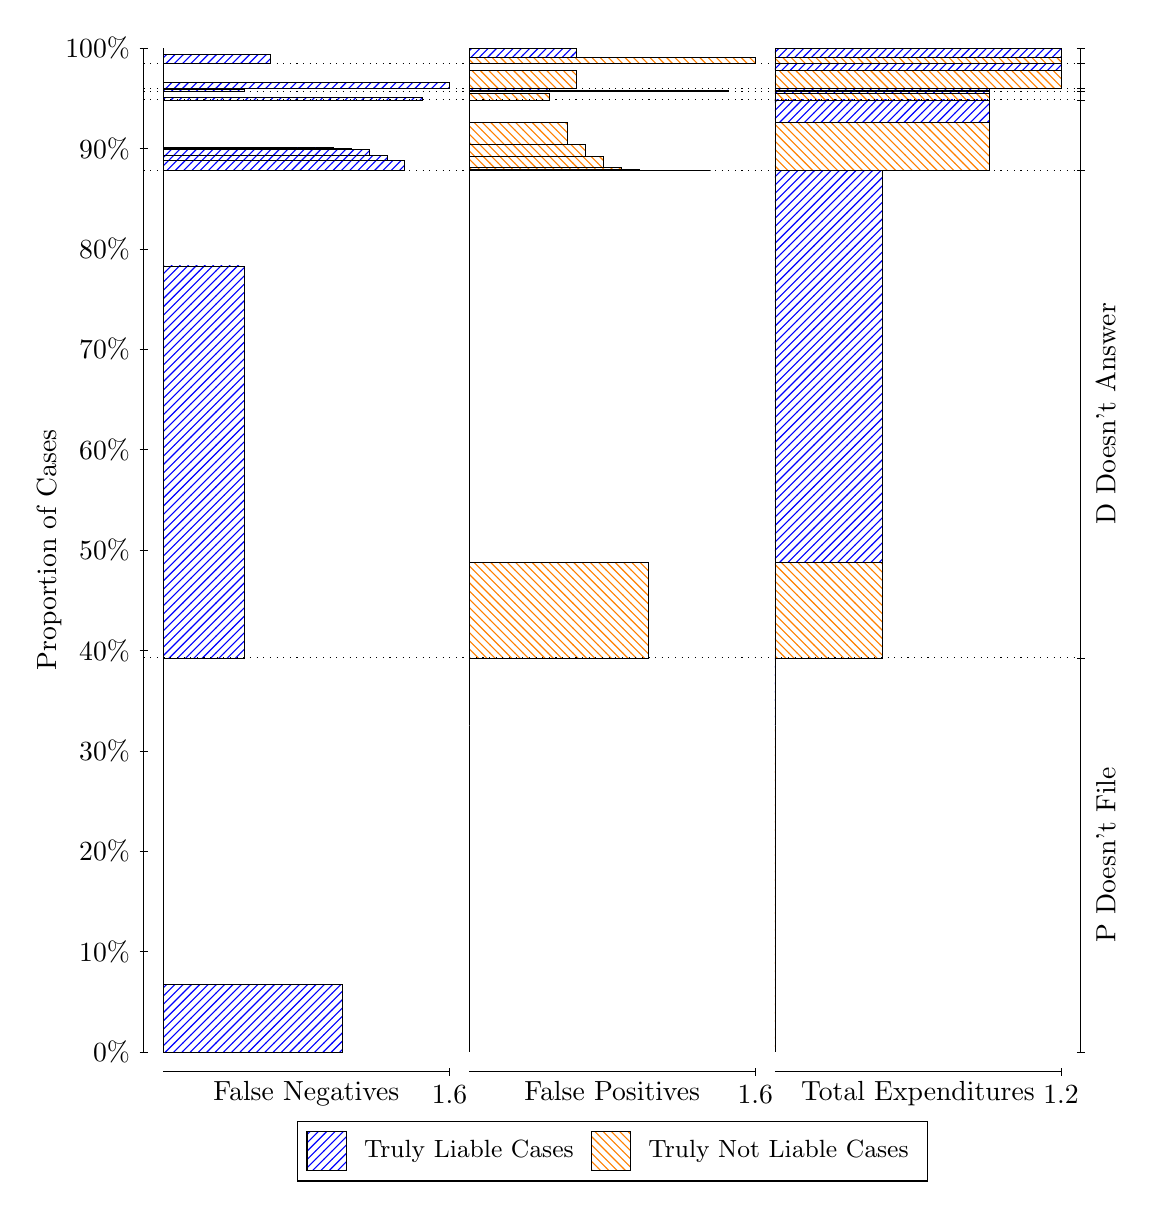
\begin{tikzpicture}
\draw[black, very thin] (1.5,1.75) -- (1.5,14.5);
\node[rotate=90, anchor=center] at (0.3, 8.125) {Proportion of Cases};
\draw[black, very thin] (1.45,1.75) -- (1.55,1.75);
\node[anchor=east] at (1.45, 1.75) {0\%};
\draw[black, very thin] (1.45,3.025) -- (1.55,3.025);
\node[anchor=east] at (1.45, 3.025) {10\%};
\draw[black, very thin] (1.45,4.3) -- (1.55,4.3);
\node[anchor=east] at (1.45, 4.3) {20\%};
\draw[black, very thin] (1.45,5.575) -- (1.55,5.575);
\node[anchor=east] at (1.45, 5.575) {30\%};
\draw[black, very thin] (1.45,6.85) -- (1.55,6.85);
\node[anchor=east] at (1.45, 6.85) {40\%};
\draw[black, very thin] (1.45,8.125) -- (1.55,8.125);
\node[anchor=east] at (1.45, 8.125) {50\%};
\draw[black, very thin] (1.45,9.4) -- (1.55,9.4);
\node[anchor=east] at (1.45, 9.4) {60\%};
\draw[black, very thin] (1.45,10.675) -- (1.55,10.675);
\node[anchor=east] at (1.45, 10.675) {70\%};
\draw[black, very thin] (1.45,11.95) -- (1.55,11.95);
\node[anchor=east] at (1.45, 11.95) {80\%};
\draw[black, very thin] (1.45,13.225) -- (1.55,13.225);
\node[anchor=east] at (1.45, 13.225) {90\%};
\draw[black, very thin] (1.45,14.5) -- (1.55,14.5);
\node[anchor=east] at (1.45, 14.5) {100\%};

\draw[black, very thin] (13.4,1.75) -- (13.4,14.5);
\draw[black, very thin] (13.35,1.75) -- (13.45,1.75);
\node[anchor=west] at (13.35, 1.75) {};
\draw[black, very thin] (13.35,6.7555) -- (13.45,6.7555);
\node[anchor=west] at (13.35, 6.7555) {};
\draw[black, very thin] (13.35,12.949) -- (13.45,12.949);
\node[anchor=west] at (13.35, 12.949) {};
\draw[black, very thin] (13.35,13.842) -- (13.45,13.842);
\node[anchor=west] at (13.35, 13.842) {};
\draw[black, very thin] (13.35,13.952) -- (13.45,13.952);
\node[anchor=west] at (13.35, 13.952) {};
\draw[black, very thin] (13.35,13.987) -- (13.45,13.987);
\node[anchor=west] at (13.35, 13.987) {};
\draw[black, very thin] (13.35,14.3) -- (13.45,14.3);
\node[anchor=west] at (13.35, 14.3) {};
\draw[black, very thin] (13.35,14.5) -- (13.45,14.5);
\node[anchor=west] at (13.35, 14.5) {};

\draw[black, very thin, pattern color=blue, pattern=north east lines] (1.75,1.75) rectangle (4.0208,2.6072);
\draw[black, very thin, pattern color=orange, pattern=north west lines] (1.75,2.6072) rectangle (1.75,6.7555);
\draw[black, very thin, pattern color=blue, pattern=north east lines] (1.75,6.7555) rectangle (2.7719,11.734);
\draw[black, very thin, pattern color=orange, pattern=north west lines] (1.75,11.734) rectangle (1.75,12.949);
\draw[black, very thin, pattern color=blue, pattern=north east lines] (1.75,12.949) rectangle (4.8156,13.07);
\draw[black, very thin, pattern color=blue, pattern=north east lines] (1.75,13.07) rectangle (4.5885,13.141);
\draw[black, very thin, pattern color=blue, pattern=north east lines] (1.75,13.141) rectangle (4.3615,13.214);
\draw[black, very thin, pattern color=blue, pattern=north east lines] (1.75,13.214) rectangle (4.1344,13.214);
\draw[black, very thin, pattern color=blue, pattern=north east lines] (1.75,13.214) rectangle (4.1344,13.23);
\draw[black, very thin, pattern color=blue, pattern=north east lines] (1.75,13.23) rectangle (3.9073,13.237);
\draw[black, very thin, pattern color=blue, pattern=north east lines] (1.75,13.237) rectangle (3.6802,13.237);
\draw[black, very thin, pattern color=blue, pattern=north east lines] (1.75,13.237) rectangle (3.4531,13.237);
\draw[black, very thin, pattern color=blue, pattern=north east lines] (1.75,13.237) rectangle (3.226,13.237);
\draw[black, very thin, pattern color=blue, pattern=north east lines] (1.75,13.237) rectangle (2.999,13.237);
\draw[black, very thin, pattern color=orange, pattern=north west lines] (1.75,13.237) rectangle (1.75,13.842);
\draw[black, very thin, pattern color=blue, pattern=north east lines] (1.75,13.842) rectangle (5.0427,13.869);
\draw[black, very thin, pattern color=orange, pattern=north west lines] (1.75,13.869) rectangle (1.75,13.952);
\draw[black, very thin, pattern color=blue, pattern=north east lines] (1.75,13.952) rectangle (2.7719,13.976);
\draw[black, very thin, pattern color=orange, pattern=north west lines] (1.75,13.976) rectangle (1.75,13.987);
\draw[black, very thin, pattern color=blue, pattern=north east lines] (1.75,13.987) rectangle (5.3833,14.067);
\draw[black, very thin, pattern color=orange, pattern=north west lines] (1.75,14.067) rectangle (1.75,14.3);
\draw[black, very thin, pattern color=blue, pattern=north east lines] (1.75,14.3) rectangle (3.1125,14.42);
\draw[black, very thin, pattern color=orange, pattern=north west lines] (1.75,14.42) rectangle (1.75,14.5);
\draw[black, very thin, pattern color=orange, pattern=north west lines] (5.6333,1.75) rectangle (5.6333,5.8983);
\draw[black, very thin, pattern color=blue, pattern=north east lines] (5.6333,5.8983) rectangle (5.6333,6.7555);
\draw[black, very thin, pattern color=orange, pattern=north west lines] (5.6333,6.7555) rectangle (7.9042,7.9713);
\draw[black, very thin, pattern color=blue, pattern=north east lines] (5.6333,7.9713) rectangle (5.6333,12.949);
\draw[black, very thin, pattern color=orange, pattern=north west lines] (5.6333,12.949) rectangle (8.699,12.949);
\draw[black, very thin, pattern color=orange, pattern=north west lines] (5.6333,12.949) rectangle (8.4719,12.949);
\draw[black, very thin, pattern color=orange, pattern=north west lines] (5.6333,12.949) rectangle (8.2448,12.949);
\draw[black, very thin, pattern color=orange, pattern=north west lines] (5.6333,12.949) rectangle (8.0177,12.949);
\draw[black, very thin, pattern color=orange, pattern=north west lines] (5.6333,12.949) rectangle (7.7906,12.957);
\draw[black, very thin, pattern color=orange, pattern=north west lines] (5.6333,12.957) rectangle (7.5635,12.982);
\draw[black, very thin, pattern color=orange, pattern=north west lines] (5.6333,12.982) rectangle (7.5635,12.982);
\draw[black, very thin, pattern color=orange, pattern=north west lines] (5.6333,12.982) rectangle (7.3365,13.126);
\draw[black, very thin, pattern color=orange, pattern=north west lines] (5.6333,13.126) rectangle (7.1094,13.279);
\draw[black, very thin, pattern color=orange, pattern=north west lines] (5.6333,13.279) rectangle (6.8823,13.555);
\draw[black, very thin, pattern color=blue, pattern=north east lines] (5.6333,13.555) rectangle (6.4281,13.555);
\draw[black, very thin, pattern color=blue, pattern=north east lines] (5.6333,13.555) rectangle (6.201,13.555);
\draw[black, very thin, pattern color=blue, pattern=north east lines] (5.6333,13.555) rectangle (5.974,13.555);
\draw[black, very thin, pattern color=blue, pattern=north east lines] (5.6333,13.555) rectangle (5.7469,13.555);
\draw[black, very thin, pattern color=blue, pattern=north east lines] (5.6333,13.555) rectangle (5.6333,13.842);
\draw[black, very thin, pattern color=orange, pattern=north west lines] (5.6333,13.842) rectangle (6.6552,13.925);
\draw[black, very thin, pattern color=blue, pattern=north east lines] (5.6333,13.925) rectangle (5.6333,13.952);
\draw[black, very thin, pattern color=orange, pattern=north west lines] (5.6333,13.952) rectangle (8.926,13.962);
\draw[black, very thin, pattern color=blue, pattern=north east lines] (5.6333,13.962) rectangle (6.6552,13.987);
\draw[black, very thin, pattern color=orange, pattern=north west lines] (5.6333,13.987) rectangle (6.9958,14.219);
\draw[black, very thin, pattern color=blue, pattern=north east lines] (5.6333,14.219) rectangle (5.6333,14.3);
\draw[black, very thin, pattern color=orange, pattern=north west lines] (5.6333,14.3) rectangle (9.2667,14.379);
\draw[black, very thin, pattern color=blue, pattern=north east lines] (5.6333,14.379) rectangle (6.9958,14.5);
\draw[black, very thin, pattern color=orange, pattern=north west lines] (9.5167,1.75) rectangle (9.5167,5.8983);
\draw[black, very thin, pattern color=blue, pattern=north east lines] (9.5167,5.8983) rectangle (9.5167,6.7555);
\draw[black, very thin, pattern color=orange, pattern=north west lines] (9.5167,6.7555) rectangle (10.879,7.9713);
\draw[black, very thin, pattern color=blue, pattern=north east lines] (9.5167,7.9713) rectangle (10.879,12.949);
\draw[black, very thin, pattern color=orange, pattern=north west lines] (9.5167,12.949) rectangle (12.242,12.949);
\draw[black, very thin, pattern color=blue, pattern=north east lines] (9.5167,12.949) rectangle (12.242,12.949);
\draw[black, very thin, pattern color=orange, pattern=north west lines] (9.5167,12.949) rectangle (12.242,13.555);
\draw[black, very thin, pattern color=blue, pattern=north east lines] (9.5167,13.555) rectangle (12.242,13.842);
\draw[black, very thin, pattern color=orange, pattern=north west lines] (9.5167,13.842) rectangle (12.242,13.842);
\draw[black, very thin, pattern color=blue, pattern=north east lines] (9.5167,13.842) rectangle (12.242,13.842);
\draw[black, very thin, pattern color=orange, pattern=north west lines] (9.5167,13.842) rectangle (12.242,13.925);
\draw[black, very thin, pattern color=blue, pattern=north east lines] (9.5167,13.925) rectangle (12.242,13.952);
\draw[black, very thin, pattern color=orange, pattern=north west lines] (9.5167,13.952) rectangle (12.242,13.962);
\draw[black, very thin, pattern color=blue, pattern=north east lines] (9.5167,13.962) rectangle (12.242,13.987);
\draw[black, very thin, pattern color=orange, pattern=north west lines] (9.5167,13.987) rectangle (13.15,14.219);
\draw[black, very thin, pattern color=blue, pattern=north east lines] (9.5167,14.219) rectangle (13.15,14.3);
\draw[black, very thin, pattern color=orange, pattern=north west lines] (9.5167,14.3) rectangle (13.15,14.379);
\draw[black, very thin, pattern color=blue, pattern=north east lines] (9.5167,14.379) rectangle (13.15,14.5);
\draw[black, dotted] (1.5,6.7555) -- (13.4,6.7555);
\draw[black, dotted] (1.5,12.949) -- (13.4,12.949);
\draw[black, dotted] (1.5,13.842) -- (13.4,13.842);
\draw[black, dotted] (1.5,13.952) -- (13.4,13.952);
\draw[black, dotted] (1.5,13.987) -- (13.4,13.987);
\draw[black, dotted] (1.5,14.3) -- (13.4,14.3);
\draw[black, very thin] (1.75,1.5) -- (5.3833,1.5);
\node[anchor=north] at (3.5667, 1.5) {False Negatives};
\draw[black, very thin] (5.3833,1.45) -- (5.3833,1.55);
\node[anchor=north] at (5.3833, 1.45) {1.6};

\draw[black, very thin] (5.6333,1.5) -- (9.2667,1.5);
\node[anchor=north] at (7.45, 1.5) {False Positives};
\draw[black, very thin] (9.2667,1.45) -- (9.2667,1.55);
\node[anchor=north] at (9.2667, 1.45) {1.6};

\draw[black, very thin] (9.5167,1.5) -- (13.15,1.5);
\node[anchor=north] at (11.333, 1.5) {Total Expenditures};
\draw[black, very thin] (13.15,1.45) -- (13.15,1.55);
\node[anchor=north] at (13.15, 1.45) {1.2};

\node[black, centered, rotate=90] at (13.72, 4.2528) {P Doesn't File};
\node[black, centered, rotate=90] at (13.72, 9.8525) {D Doesn't Answer};






\draw (7.449999999999999,1.5) node[draw=none] (baseCoordinate) {};
\begin{scope}[align=center]
        \matrix[scale=0.5, draw=black, below=0.5cm of baseCoordinate, nodes={draw}, column sep=0.1cm]{
            \node[rectangle, draw, minimum width=0.5cm, minimum height=0.5cm, pattern=north east lines, pattern color=blue] {}; &
            \node[draw=none, font=\small] (B) {Truly Liable Cases}; &
            \node[rectangle, draw, minimum width=0.5cm, minimum height=0.5cm, pattern=north west lines, pattern color=orange] {}; &
            \node[draw=none, font=\small] (B) {Truly Not Liable Cases}; \\
            };
\end{scope}

\end{tikzpicture}
\end{document}